\newcommand{\bassangPrjSemestre}{Docker and Internet of Things (travail de semestre)}
\newcommand{\bassangPrjBachelor}{Docker and Internet of Things (travail de Bachelor)}
\section{Introduction}

Le but de ce chapitre est d'apporter un contexte au projet réalisé afin de comprendre ce qui est expliqué dans la suite de ce document. Si le lecteur souhaite connaître les tréfonds de Docker, il est recommandé de lire le rapport "\bassangPrjSemestre" de M. Loic Bassang \cite{TODO}. 

Docker est un outil qui permet de empaqueter une application et ses dépendances dans un container léger, auto-suffisant, isolé et portable. En intégrant leur application dans un container, les développeurs s'assurent que celle-ci va tourner sur n'importe quel environnement GNU/Linux. Ainsi, le temps passé à configurer les différents environnements (développement, test et production typiquement) est réduit voire même unifié.
TODO: citer \url{https://en.wikipedia.org/wiki/Docker_%28software%29}, \url{https://www.linux.com/news/docker-shipping-container-linux-code}, \url{https://www.docker.com/what-docker}

Les caractéristiques principales des containers Docker sont les suivantes :
\begin{itemize}
\item \textit{légers} : les containers partagent le même kernel et librairies que le système d'exploitation hôte permettant ainsi un démarrage rapide des containers et une utilisation mémoire contenue
\item \textit{isolés} : les containers sont isolés grâce à des mécanismes offerts par le kernel. Voir section \ref{pres-docker-isolation} pour plus de détails
\item \textit{éphémères et maintenables} : les containers sont conçus pour être créés et détruits régulièrement contrairement à un serveur ou une machine virtuelle pour lesquels un arrêt est souvent critique. Ils sont maintenables dans le sens où il est possible de revenir à une version précédente facilement et qu'il est aisé de déployer une nouvelle version
\end{itemize}

Les sections qui suivent abordent un peu plus en profondeur certains points clés de Docker qui ont été jugées importantes.

\section{Containers vs machines virtuelles}
Suite à la lecture de la section précédente, il serait normal de se dire que ces containers partagent certaines caractéristiques avec les machines virtuelles.

Voici les différences majeures qu'il existe entre les containers et les machines virtuelles.

\begin{figure}[hbtp]
\centering
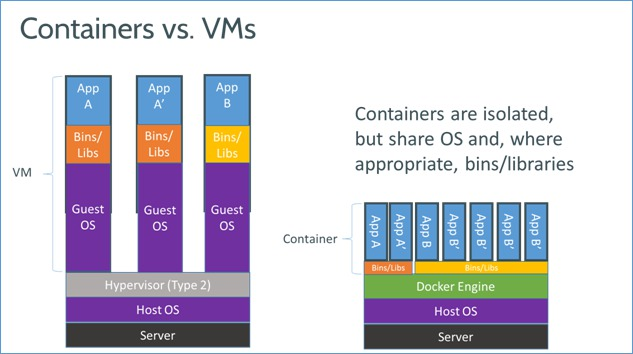
\includegraphics[scale=0.5]{img/containers_vs_vm.png}
\caption{Containers vs machines virtuelles}
\end{figure}

Les machines virtuelles possèdent leur propre OS qui embarque ses propres binaires et librairies. Ceci engendre une perte d'espace disque importante surtout si les binaires ou libraires sont communes à plusieurs machines virtuelles. De plus, démarrer une machine virtuelle prend du temps (jusqu'à plusieurs minutes). En outre, les machines virtuelles doivent installer leurs propres drivers afin de communiquer avec l'hyperviseur (logiciel s'exécutant à l'intérieur d'un OS hôte qui gère les machines virtuelles). Un avantage cependant est l'isolation complète d'une machine virtuelle qui ne peut communiquer avec les autres par défaut.

Les containers s'exécutent de manière isolée par dessus l'OS hôte qui partage ses ressources (kernel, binaires, librairies, périphériques,...). Plus légers, les containers démarrent en quelques secondes seulement. Sur une machine, il est tout à fait possible de lancer de milliers de containers similaires car l'empreinte mémoire est réduite et l'espace disque occupé est partagé si les containers sont semblables. Ceci est expliqué plus en détail à la section \ref{pres-docker-systeme-fichiers-couches}. Les containers sont isolés mais ils peuvent aussi communiquer entre eux si on leur a explicitement donner l'autorisation.

Si le lecteur désire connaître plus de détails concernant la virtualisation, il est conseillé de lire le chapitre 3.2 du rapport "\bassangPrjSemestre" de M. Loic Bassang \cite{TODO} qui amène une bonne introduction aux différents types de virtualisation.


\section{Docker images et Docker containers}
Avec Docker, une application est encapsulée avec toutes ses dépendances et sa configuration dans une \textbf{image}. 

Pour construire cette image, on utilise un Dockerfile. Il s'agit d'un fichier qui décrit les étapes de création et de configuration qu'il faut faire pour obtenir l'application configurée. C'est dans ce fichier qu'on retrouve l'OS à utiliser, les dépendances à installer et toutes autres configurations utiles au bon fonctionnement de l'application à déployer. 

Typiquement un Dockerfile permettant de lancer un serveur web Nginx qui affiche un "hello world" ressemble à ceci :

\begin{bashcode}
FROM alpine  # image de départ
MAINTAINER support@tutum.co  # mainteneur du Dockerfile
RUN apk --update add nginx php-fpm && \  # installation des dépendances
    mkdir -p /var/log/nginx && \
    touch /var/log/nginx/access.log && \
    mkdir -p /tmp/nginx && \
    echo "clear_env = no" >> /etc/php/php-fpm.conf
ADD www /www  # ajout des sources de l'application
ADD nginx.conf /etc/nginx/  # ajout d'un fichier de configuration
EXPOSE 80  # ouverture du port 80
CMD php-fpm -d variables_order="EGPCS" && (tail -F /var/log/nginx/access.log &) && exec nginx -g "daemon off;" # commande à lancer au lancement du container
\end{bashcode}

Source: \url{https://github.com/tutumcloud/hello-world/blob/master/Dockerfile}

Un Dockerfile est en quelque sorte la recette de cuisine qui permet de construire une image Docker.

Une fois l'image construite, on peut exécuter l'application dans un container. Un container Docker est donc une instance de l'image fraîchement créée. La figure \ref{docker-dockerfile-image-container} montre les relations entre un Dockerfile, une image et un container.

\begin{figure}[hbtp]
\centering
\includegraphics[scale=0.7]{img/docker-dockerfile-image-container.png}
\caption{Dockerfile, image et container}
\label{docker-dockerfile-image-container}
\end{figure}


\section{Système de fichiers en couche}\label{pres-docker-systeme-fichiers-couches}
Chaque image Docker est composée d'une liste de couches (\textit{layers}) superposées en lecture seule. Chaque couche représente la différence du système de fichiers par rapport à la couche précédente. Sur la figure \ref{docker-image-layers}, on peut voir 4 couches (identifiables avec des ID) et leur taille respectives.

\begin{figure}[hbtp]
\centering
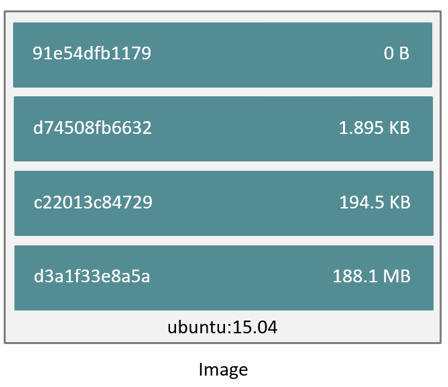
\includegraphics[scale=0.8]{img/image-layers}
\caption{Couches d'une image Docker}
\label{docker-image-layers}
\end{figure}

A la création d'un container, une nouvelle couche fine est ajoutée. Cette couche, appelée "container layer" est accessible en écriture durant l'exécution du container. La figure \ref{docker-container-layers} le montre clairement.

\begin{figure}[hbtp]
\centering
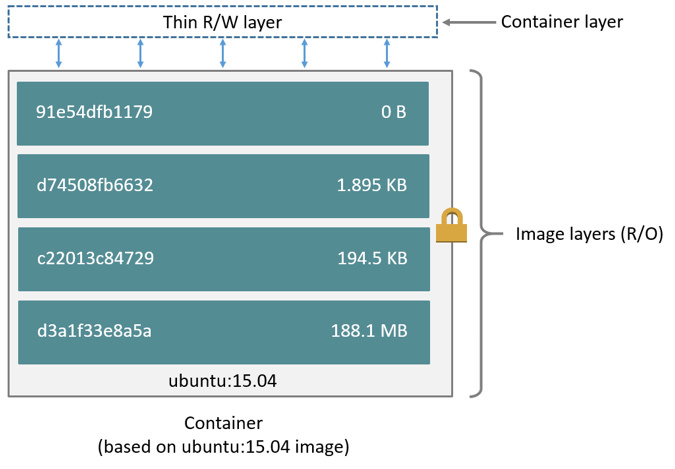
\includegraphics[scale=0.8]{img/container-layers}
\caption{Couches d'un container Docker}
\label{docker-container-layers}
\end{figure}

Un mot supplémentaire sur une nouvelle caractéristiques arrivée avec Docker 1.10 (mars 2016); avant cette version, Docker attribuait des UUID\footnote{UUID : \url{https://fr.wikipedia.org/wiki/Universal_Unique_Identifier}} générés aléatoirement pour identifier les couches d'une image. Désormais, ces UUID sont remplacés par des hash appelés \textit{secure content hash}.

Les différences principales entre un UUID et un hash sont :
\begin{itemize}
\item Un UUID est généré aléatoirement, donc deux images exactement identiques auront un UUID différent alors qu'en utilisant un hash, le résultat sera identique
\item Les UUID, même si la probabilité est rare\footnote{Probabilité de doublon : \url{https://en.wikipedia.org/wiki/Universally_unique_identifier\#Random_UUID_probability_of_duplicates}}, il est possible de générer deux fois le même UUID ce qui peut poser des problèmes lors de la construction des images
\item Une image téléchargée chez une personne A aura un UUID différent que la même image téléchargée chez une personne B. Impossible de s'assurer de l'intégrité de l'image téléchargée en se basant sur l'UUID. En utilisant le hash, on s'assure du même résultat si l'image est identique
\end{itemize}

Par conséquent Docker avance les avantages suivants:
\begin{itemize}
\item Intégrité des images téléchargées et envoyées (sur Docker Hub par exemple)
\item Évite les collisions lors de l'identification des images et des couches
\item Permet de partager des couches identiques qui proviendraient de \textit{build} différents
\end{itemize}

Le dernier point est relativement intéressant. En effet, si deux images de base (Ubuntu et Debian) sont différentes mais qu'une couche supérieure est identique (par exemple l'ajout d'un même fichier texte) alors cette couche supérieure peut être partagée entre les deux images (puisqu'elle possède le même hash). Ceci peut potentiellement offrir un gain d'espace disque conséquent si plusieurs images partagent plusieurs couches identiques. Ceci n'aurait pas pu être possible avec les UUID car les deux couches auraient produit deux UUID différents. Un exemple est visible à la figure \ref{shared-layer-hash}

\begin{figure}[hbtp]
\centering
\includegraphics[scale=0.7]{img/shared-layer-hash}
\caption{Couche partagée entre deux images Docker}
\label{shared-layer-hash}
\end{figure}

D'autres explications plus détaillées sur le système de fichiers en couches sont disponible au chapitre 5.4.1 ont fait l'objet d'un chapitre dans le rapport "\bassangPrjSemestre" de M. Loic Bassang.


\section{Isolation}\label{pres-docker-isolation}
TODO dire à quels niveaux Docker est isolé, parler des namespaces et des cgroups


\section{Contraintes liées au monde de l'embarqué}
TODO décrire les problématiques du monde embarqué, dire comment on peut en résoudre avec Docker et les pré-requis nécessaires pour utiliser Docker sur un système embarqué.